% \documentclass[handout]{beamer}
\documentclass{beamer}
\mode<presentation>
{
  \usetheme{Warsaw}
  % \setbeamercovered{transparent}
  \useoutertheme{infolines}

}

\usepackage[italian]{babel}
\usepackage[utf8]{inputenc}
\usepackage{wrapfig}
\usepackage[T1]{fontenc}
\usepackage{float}
\usepackage{multicol}
\usepackage{blindtext}
\usepackage{mwe}

\definecolor{nord1}{RGB}{46, 52, 64} 
\definecolor{nord2}{RGB}{76, 105, 141} 
\definecolor{nord3}{RGB}{94, 129, 172}
\definecolor{nord4}{RGB}{129, 161, 193} 
\definecolor{nord5}{RGB}{136, 192, 208}  
\definecolor{nord6}{RGB}{163, 190, 140}
\definecolor{nord7}{RGB}{191, 97, 106}
\definecolor{nordred}{RGB}{191, 97, 106}
\definecolor{nordgreen}{RGB}{135, 157, 116}

\setbeamercolor{palette primary}{bg=nord2,fg=white}
\setbeamercolor{palette secondary}{bg=nord3,fg=white}
\setbeamercolor{palette tertiary}{bg=nord4,fg=white}

\setbeamercolor{block title}{bg=nord2,fg=white}

\setbeamercolor{itemize item}{fg=nord3}
\setbeamercolor{itemize subitem}{fg=nord4}
\setbeamercolor{itemize subsubitem}{fg=nord5}

\setbeamertemplate{itemize item}[square]
\setbeamertemplate{itemize subitem}[circle]
\setbeamertemplate{itemize subsubitem}[triangle]

\usecolortheme[named=nord2]{structure}

\title[] {RLPBWT}

% \subtitle
% {Presentation Subtitle} % (optional)

\author[] {Davide Cozzi}


\institute[] {Dipartimento di Informatica, Sistemistica e Comunicazione
  (DISCo)\\
  Università degli Studi di Milano Bicocca}

\date[] {}

\subject{Presentation}
\pgfdeclareimage[height=0.5cm]{university-logo}{img/logo_unimib.pdf}
\logo{\pgfuseimage{university-logo}}

\AtBeginSection[]
{
  \begin{frame}<beamer>{Outline}
    \tableofcontents[currentsection, currentsubsection]
  \end{frame}
}


% If you wish to uncover everything in a step-wise fashion, uncomment
% the following command: 

% \beamerdefaultoverlayspecification{<+->}


\begin{document}

\begin{frame}
  \titlepage
\end{frame}

\begin{frame}{Outline}
  \setcounter{tocdepth}{1}
  \tableofcontents
\end{frame}

\section{RLPBWT}
\begin{frame}{Some definitions}
  \begin{block}{The permutation, panel $M$, $n\times m$}
    In \textit{RLPBWT} we have a permutation $\pi_j$, $\forall\,\, 1\leq j\leq
    m$ that stably sorts the bits of the $j$-th column of the PBWT.\\
    This permutation can be stored in space
    proportional to the number of runs in the $j$-th column of the PBWT
  \end{block}
  \pause
  \begin{block}{}
    The positions in the columns of the PBWT of the bits in the $i$-th row of
    $M$ are:
    \pause
    \[i, \pi_1(i), \pi_2(\pi_1(i)),\ldots, \pi_{m-1}(\cdots(
      \pi_2(\pi_1(i)))\cdots)\] 
  \end{block}
  \begin{block}{}
    Extracting the bits of the $i$-th row of $M$ reduces to iteratively applying
    the $\pi_{m-1}$ permutations, corresponding to iteratively apply LF in a
    standard BWT 
  \end{block}
\end{frame}
\begin{frame}{The permutation}
  \begin{block}{Computing the permutation}
    \[\pi_j(p)=
      \begin{cases}
        p-count_1 &\mbox{if } column[pref[p]]=0\\
        count_0+count_1-1 &\mbox{if } column[pref[p]]=1\\
      \end{cases}
    \]
    \begin{itemize}
      \item $count_0$: total number of zeros in the PBWT column
      \item $count_1$: number of ones in the PBWT column as far as index $p$
    \end{itemize}
  \end{block}
  \begin{block}{``LF-mapping'' in Durbin's algorithm}
    \[w(i,\sigma)=
      \begin{cases}
        u[i]&\mbox{if } \sigma=0\\
        c+v[i]&\mbox{if } \sigma=1\\
      \end{cases}
    \]
    \begin{itemize}
      \item $c$: total number of zeros in the column
      \item $u[i]$: number of zeros in the column as far as index $i$
      \item $v[i]$: number of ones in the column as far as index $i$
    \end{itemize}
  \end{block}
\end{frame}
\begin{frame}{Travis's example}
  \begin{figure}[H]
    \centering
    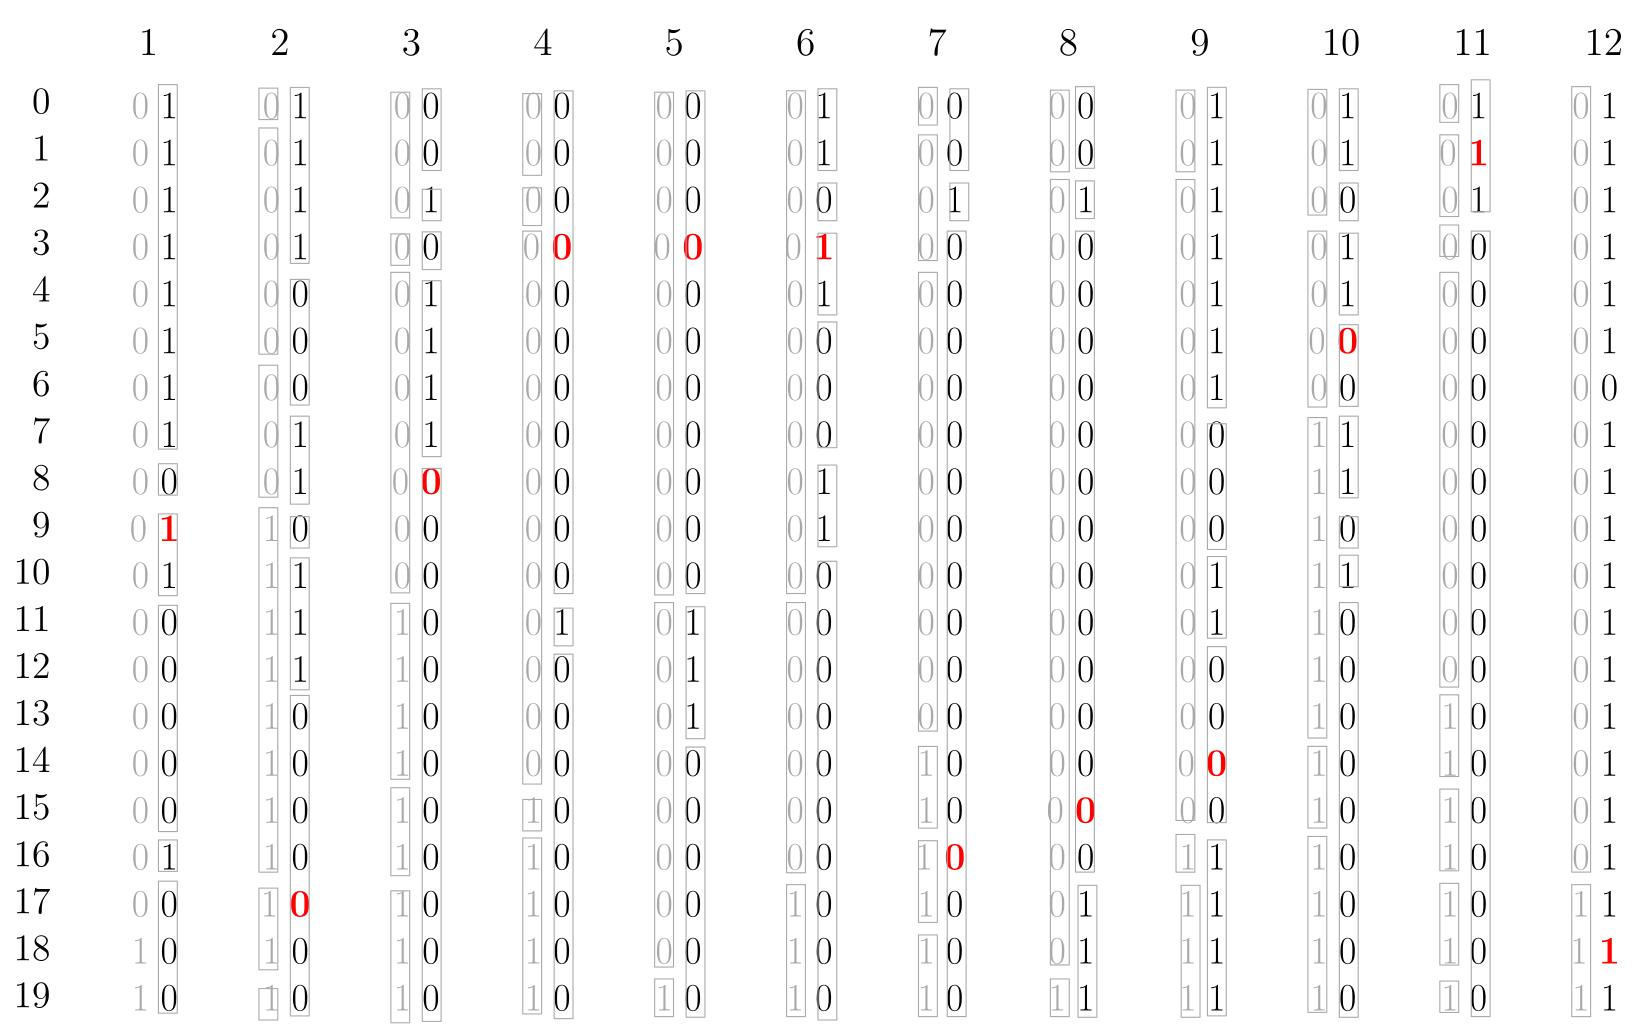
\includegraphics[scale = 0.2]{img/trick.jpg}
  \end{figure}
\end{frame}
\begin{frame}{The compressed data structure}
  \begin{block}{The tables}
    \begin{itemize}
      \item a set of $m$ tables in which the $m$-th table stores only the
      positions of the run-heads in the $m$-th column and a bool to check the
      first symbol: 0 or 1
      \item the $i$-th row of the $j$-th table stores a quadruple
    \end{itemize}    
  \end{block}
  \pause
  \begin{block}{The quadruple}
    \begin{enumerate}
      \item the position $p$ of the $i$-th run-head in the $j$-th column of the
      PBWT 
      \item the permutation $\pi_j(p)$
      \item the index of the run containing bit $\pi_j(p)$ in the $(j + 1)$-st
      column of the PBWT
      \item the threshold, that's the index of the minimum \textit{LCP value}
      (current column minus divergence array value) in the run
    \end{enumerate}
  \end{block}
\end{frame}
\begin{frame}{Row extraction}
  \begin{block}{First step}
    We start by finding the row of the first table that starts with the position
    $p$ of the head of the run containing bit $i$ in first column of the PBWT,
    computing: 
    \pause
    \[\pi_1(i)=\pi_1(p)+i-p\]
    \pause
    looking up the row for the run containing bit $\pi_1(p)$ in the the second
    table and scanning down the table until we find the row for the run
    containing bit $\pi_1(i)$ 
  \end{block}
  \begin{block}{Next step}
    We continue repeating this procedure for each column
  \end{block}
\end{frame}
\begin{frame}{Travis's example I}
  \begin{figure}[H]
    \centering
    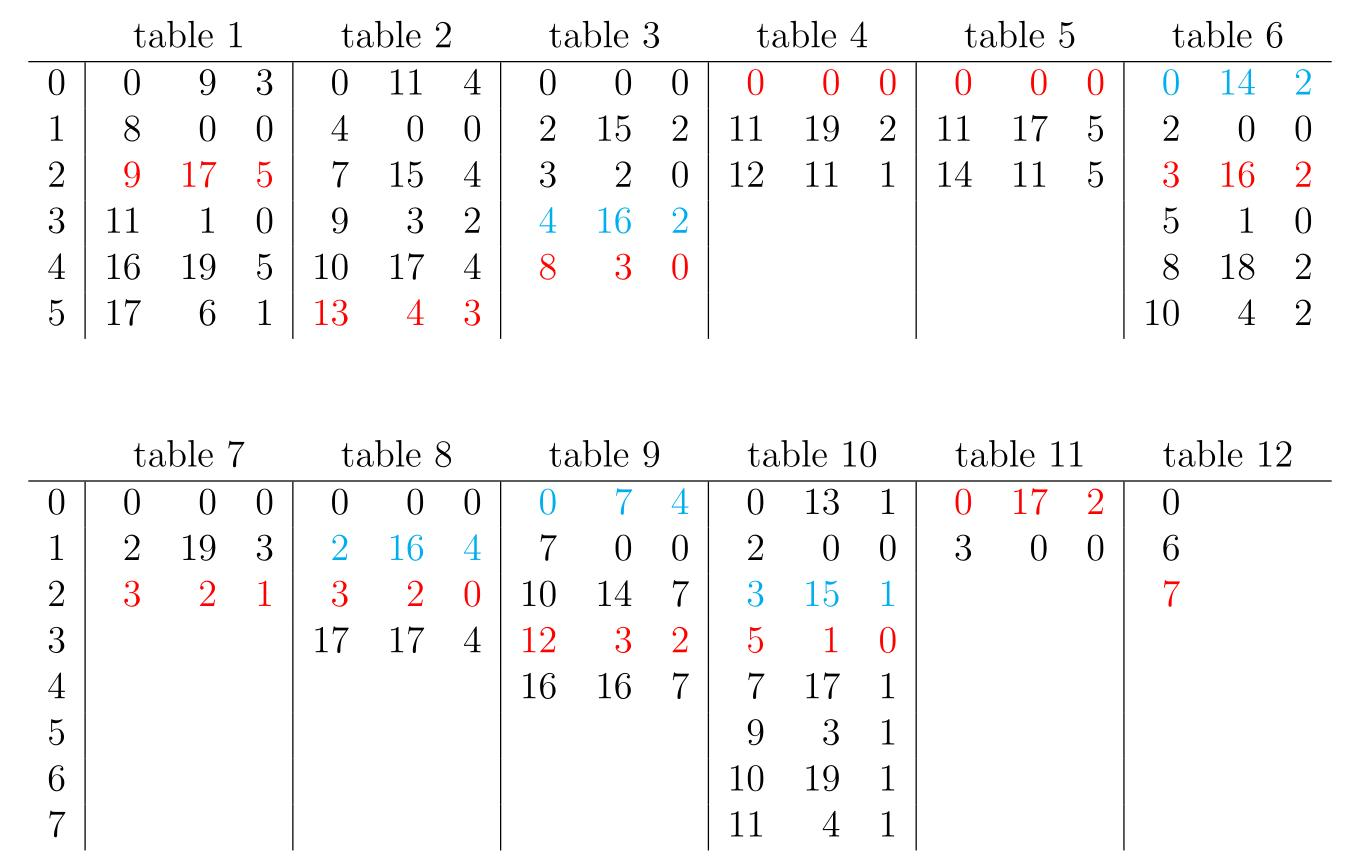
\includegraphics[scale = 0.22]{img/trick2.jpg}
  \end{figure}
\end{frame}
\begin{frame}{Travis's example II}
  \begin{block}{Extraction of row 9, $\pi_j(i)=\pi_j(p)+i-p$}
    \begin{multicols}{2}
      \begin{itemize}
        \item $\pi_1(9)=17+9-9=17$
        \item $\pi_2(17)=4+17-13=8$
        \item $\pi_3(8)=4+8-8=3$
        \item $\pi_4(3)=0+3-0=3$
        \item $\pi_5(3)=0+3-0=3$
        \item $\pi_6(3)=16+3-3=16$

        \item $\pi_7(16)=2+16-3=15$
        \item $\pi_8(15)=2+15-3=14$
        \item $\pi_9(14)=3+14-12=5$
        \item $\pi_{10}(5)=1+5-5=1$
        \item $\pi_{11}(1)=17+1-0=18$
        %\item $\pi_{12}(3)=16+3-3=16$        
      \end{itemize}
    \end{multicols}
  \end{block}
\end{frame}
\section{Example}
\begin{frame}{The matrixes}
  \begin{block}{Panel and query}
    \begin{table}[H]
      \centering
      \tiny
      \begin{tabular}{c|c|c|c|c|c|c|c|c|c|c|c|c|c|c|c|c|c|c|c}
        \hline
        0 & 1 & 2 & 3 & 4 & 5 & 6 & 7 & 8 & 9 & 10 & 11 & 12 & 13 & 14 & 15 & 16
        & 17 & 18 & 19\\
        \hline
        \hline
        
        1 & 1 & 0 & 1 & 0 & 0 & 1 & 1 & 1 & 1 & 1 & 0 & 0 & 1 & 0 & 0 & 1 & 0
             & 0 & 1\\
        0 & 1 & 0 & 0 & 0 & 0 & 1 & 1 & 1 & 1 & 1 & 0 & 0 & 1 & 1 & 1 & 0 & 0
             & 1 & 0\\
        0 & 0 & 0 & 1 & 0 & 0 & 0 & 0 & 0 & 1 & 1 & 1 & 1 & 0 & 0 & 0 & 1 & 0
             & 1 & 0\\
        1 & 0 & 0 & 1 & 1 & 0 & 1 & 0 & 1 & 0 & 0 & 0 & 1 & 1 & 1 & 0 & 0 & 0
             & 1 & 0\\
        0 & 1 & 1 & 0 & 1 & 1 & 1 & 1 & 1 & 0 & 0 & 1 & 0 & 0 & 1 & 1 & 1 & 1
             & 0 & 0\\
        1 & 1 & 0 & 0 & 1 & 0 & 1 & 0 & 1 & 0 & 1 & 0 & 1 & 0 & 0 & 0 & 1 & 1
             & 1 & 1\\
        0 & 0 & 0 & 1 & 0 & 1 & 1 & 1 & 1 & 1 & 1 & 1 & 0 & 0 & 1 & 0 & 0 & 0
             & 1 & 1\\
        \hline
        \hline
        \hline
        0 & 0 & 1 & 0 & 1 & 1 & 1 & 1 & 1 & 1 & 1 & 0 & 0 & 1 & 0 & 0 & 0 & 1
             & 1 & 1
      \end{tabular}
    \end{table}
  \end{block}
  \begin{block}{PBWT Matrix}
    \begin{table}[H]
      \centering
      \tiny
      \begin{tabular}{c|c|c|c|c|c|c|c|c|c|c|c|c|c|c|c|c|c|c|c}
        \hline
        0 & 1 & 2 & 3 & 4 & 5 & 6 & 7 & 8 & 9 & 10 & 11 & 12 & 13 & 14 & 15 & 16
        & 17 & 18 & 19\\
        \hline
        \hline
        1 & 1 & 0 & 1 & 0 & 0 & 1 & 0 & 0 & 1 & 1 & 0 & 1 & 1 & 1 & 0 & 1 & 0
             & 1 & 1 \\
        0 & 0 & 0 & 1 & 1 & 0 & 0 & 1 & 1 & 0 & 0 & 1 & 1 & 1 & 1 & 0 & 1 & 0
             & 1 & 0 \\
        0 & 1 & 0 & 1 & 1 & 1 & 1 & 1 & 1 & 0 & 0 & 0 & 0 & 0 & 0 & 0 & 1 & 0
             & 1 & 1 \\
        1 & 0 & 0 & 0 & 0 & 0 & 1 & 0 & 1 & 1 & 1 & 1 & 0 & 0 & 0 & 1 & 0 & 1
             & 1 & 0 \\
        0 & 1 & 1 & 1 & 0 & 0 & 1 & 0 & 1 & 1 & 1 & 0 & 0 & 1 & 1 & 0 & 0 & 0
             & 0 & 0 \\
        1 & 0 & 0 & 0 & 1 & 1 & 1 & 1 & 1 & 1 & 1 & 0 & 1 & 0 & 0 & 1 & 1 & 0
             & 1 & 0 \\
        0 & 1 & 0 & 0 & 0 & 0 & 1 & 1 & 1 & 0 & 1 & 1 & 0 & 0 & 1 & 0 & 0 & 1
             & 0 & 1 \\
        \hline
      \end{tabular}
    \end{table}
  \end{block}
\end{frame}
\begin{frame}{Prefix and Divergence Arrays}
  \begin{block}{Prefix Arrays}
    \begin{table}[H]
      \tiny
      \begin{tabular}{c|c|c|c|c|c|c|c|c|c|c|c|c|c|c|c|c|c|c|c}
        \hline
        0 & 1 & 2 & 3 & 4 & 5 & 6 & 7 & 8 & 9 & 10 & 11 & 12 & 13 & 14 & 15 & 16
        & 17 & 18 & 19\\
        \hline
        \hline
        0 & 1 & 2 & 2 & 1 & 1 & 1 & 2 & 2 & 2 & 5 & 3 & 3 & 1 & 4 & 5 & 5 & 6
             & 6 & 0\\  
        1 & 2 & 6 & 6 & 5 & 2 & 2 & 1 & 5 & 5 & 3 & 4 & 5 & 0 & 6 & 2 & 2 & 3
             & 3 & 4\\  
        2 & 4 & 3 & 3 & 4 & 6 & 0 & 0 & 3 & 3 & 4 & 5 & 1 & 4 & 5 & 0 & 0 & 1
             & 1 & 6\\  
        3 & 6 & 1 & 1 & 2 & 0 & 5 & 5 & 1 & 1 & 2 & 2 & 0 & 6 & 2 & 4 & 6 & 5
             & 2 & 3\\  
        4 & 0 & 4 & 0 & 6 & 5 & 3 & 3 & 0 & 0 & 1 & 1 & 4 & 3 & 1 & 6 & 3 & 2
             & 0 & 1\\  
        5 & 3 & 0 & 5 & 3 & 4 & 6 & 6 & 6 & 6 & 0 & 0 & 2 & 5 & 0 & 1 & 4 & 0
             & 5 & 2\\
        6 & 5 & 5 & 4 & 0 & 3 & 4 & 4 & 4 & 4 & 6 & 6 & 6 & 2 & 3 & 3 & 1 & 4
             & 4 & 5\\
        \hline
      \end{tabular}
    \end{table}
  \end{block}
  \begin{block}{LCP Arrays: current \textit{k} minus the original Durbin's
      divergence arrays}  
    \begin{table}[H]
      \tiny
      \begin{tabular}{c|c|c|c|c|c|c|c|c|c|c|c|c|c|c|c|c|c|c|c}
        \hline
        0 & 1 & 2 & 3 & 4 & 5 & 6 & 7 & 8 & 9 & 10 & 11 & 12 & 13 & 14 & 15 & 16
        & 17 & 18 & 19\\
        \hline
        \hline
        0 & 0 & 0 & 0 & 0 & 0 & 0 & 0 & 0 & 0 & 0 & 0 & 0 & 0 & 0 & 0 & 0 & 0
             & 0 & 0 \\
        0 & 1 & 2 & 3 & 3 & 1 & 2 & 0 & 1 & 0 & 6 & 3 & 1 & 9 & 3 & 3 & 4 & 3
             & 4 & 1 \\
        0 & 1 & 1 & 2 & 1 & 5 & 4 & 3 & 4 & 5 & 2 & 0 & 2 & 1 & 1 & 1 & 2 & 1
             & 2 & 0 \\
        0 & 1 & 0 & 1 & 0 & 3 & 1 & 2 & 0 & 1 & 0 & 1 & 8 & 2 & 2 & 0 & 1 & 0
             & 1 & 5 \\
        0 & 0 & 2 & 2 & 4 & 0 & 2 & 3 & 4 & 5 & 1 & 2 & 0 & 0 & 0 & 4 & 2 & 5
             & 4 & 3 \\
        0 & 1 & 1 & 3 & 3 & 2 & 0 & 1 & 2 & 3 & 6 & 7 & 1 & 2 & 10 & 1 & 0 & 3
             & 0 & 2 \\
        0 & 1 & 2 & 0 & 2 & 1 & 1 & 2 & 3 & 4 & 4 & 5 & 3 & 1 & 1 & 2 & 2 & 1
             & 2 & 1\\
      \end{tabular}
    \end{table}
  \end{block}
\end{frame}

\begin{frame}{Run-Length PBWT I, \textit{p, perm, next perm, threshold}}
  \begin{block}{ $[0,1,2,3,4]$} 
    {\footnotesize{\[
          \begin{matrix}
            0 & 4 & 4 & 0\\
            1 & 0 & 0 & 1\\
            3 & 5 & 5 & 3\\
            \color{nordgreen} 4 &\color{nordgreen} 2 &\color{nordgreen} 2
            &\color{nordgreen} 4\\ 
            5 & 6 & 6 & 5\\
            6 & 3 & 3 & 6
          \end{matrix}
          \Longrightarrow
          \begin{matrix}
            0 & 3 & 0 & 0\\
            1 & 0 & 0 & 1\\
            \color{nordgreen} 2 &  \color{nordgreen} 4 &  \color{nordgreen} 1 &
            \color{nordgreen} 2\\
            3 & 1 & 0 & 3\\
            4 & 5 & 2 & 4\\
            5 & 2 & 0 & 5\\
            6 & 6 & 2 & 6
          \end{matrix}
          \Longrightarrow
          \begin{matrix}
            0 & 0 & 0 & 0\\
            \color{nordgreen} 4 & \color{nordgreen} 6 & \color{nordgreen} 3 &
            \color{nordgreen} 4\\
            5 & 4 &  2 & 5
          \end{matrix}
          \Longrightarrow
          \begin{matrix}
            0 & 3 & 2 & 0\\
            3 & 0 & 0 & 3\\
            4 & 6 & 4 & 4\\
            \color{nordgreen} 5 & \color{nordgreen} 1 & \color{nordgreen} 1 &
            \color{nordgreen} 6
          \end{matrix}
          \Longrightarrow
          \begin{matrix}
            0 & 0 & 0 & 0\\
            \color{nordgreen} 1 &  \color{nordgreen} 4 &  \color{nordgreen} 2 &
            \color{nordgreen} 2\\
            3 & 1 & 0 & 3\\
            5 & 6 & 4 & 5\\
            6 & 3 & 2 & 6
          \end{matrix}\]}}
  \end{block}
  \begin{block}{$[5,6,7,8,9]$}
    {\footnotesize{\[
          \begin{matrix}
            0 & 0 & 0 & 0\\
            2 & 5 & 2 & 2\\
            \color{nordred} 3 & \color{nordred} 2 & \color{nordred} 2 &
            \color{nordred} 4\\
            \color{nordgreen} 5 &  \color{nordgreen} 6 &   \color{nordgreen}2 &
            \color{nordgreen} 5\\
            6 & 4 & 2 & 6
          \end{matrix}
          \Longrightarrow
          \begin{matrix}
            0 & 1 & 1 & 0\\
            1 & 0 & 0 & 1\\
            \color{nordgreen} 2 & \color{nordgreen} 2 & \color{nordgreen} 1 &
            \color{nordgreen} 5
          \end{matrix}
          \Longrightarrow
          \begin{matrix}
            0 & 0 & 0 & 0\\
            \color{nordred} 1 &  \color{nordred} 3 &  \color{nordred} 1 &
            \color{nordred} 1\\ 
            3 & 1 & 1 & 3\\
            \color{nordgreen} 5 & \color{nordgreen} 5 & \color{nordgreen} 1 &
            \color{nordgreen} 5
          \end{matrix}
          \Longrightarrow
          \begin{matrix}
            0 & 0 & 0 & 0\\
            \color{nordgreen} 1 & \color{nordgreen} 1 & \color{nordgreen} 1 &
            \color{nordgreen} 3
          \end{matrix}
          \Longrightarrow
          \begin{matrix}
            0 & 3 & 2 & 0\\
            \color{nordred} 1 &  \color{nordred} 0 &  \color{nordred} 0 &
            \color{nordred} 1\\ 
            3 & 4 & 2 & 3\\
            \color{nordgreen} 6 & \color{nordgreen} 2 & \color{nordgreen} 1 &
            \color{nordgreen} 6           
          \end{matrix}\]}}
  \end{block}
\end{frame}
\begin{frame}{Run-Length PBWT II}
  \begin{block}{$[10,11,12,13,14]$}
    {\footnotesize{\[
          \begin{matrix}
            0 & 2 & 2 & 0\\
            \color{nordgreen} 1 & \color{nordgreen} 0 & \color{nordgreen} 0 &
            \color{nordgreen} 2\\
            3 & 3 & 3 & 3
          \end{matrix}
          \Longrightarrow
          \begin{matrix}
            \color{nordred} 0 & \color{nordred} 0 & \color{nordred} 0 &
            \color{nordred} 0\\
            \color{nordgreen} 1 & \color{nordgreen} 4 & \color{nordgreen} 1 &
            \color{nordgreen} 1\\
            2 & 1 & 0 & 2\\
            3 & 5 & 2 & 3\\
            4 & 2 & 1 & 4\\
            6 & 6 & 3 & 6
          \end{matrix}
          \Longrightarrow
          \begin{matrix}
            0 & 4 & 2 & 0\\
            \color{nordgreen} 2 & \color{nordgreen} 0 & \color{nordgreen} 0 &
            \color{nordgreen} 4\\
            5 & 6 & 3 & 5\\
            6 & 3 & 1 & 6
          \end{matrix}
          \Longrightarrow
          \begin{matrix}
            \color{nordred} 0 & \color{nordred} 4 & \color{nordred} 2 &
            \color{nordred} 0\\
            \color{nordgreen} 2 & \color{nordgreen} 0 & \color{nordgreen} 0 &
            \color{nordgreen}2\\ 
            4 & 6 & 4 & 4\\
            5 & 2 & 1 & 6
          \end{matrix}
          \Longrightarrow
          \begin{matrix}
            \color{nordgreen} 0 & \color{nordgreen} 3 & \color{nordgreen} 1 &
            \color{nordgreen} 0\\ 
            2 & 0 & 0 & 2\\
            4 & 5 & 3 & 4\\
            5 & 2 & 0 & 5\\
            6 & 6 & 4 & 6
          \end{matrix}\]}}
  \end{block}
  \begin{block}{$[15,16,17,18,19]$}
    {\footnotesize{\[
          \begin{matrix}
            0 & 0 & 0 & 0\\
            \color{nordgreen} 3 & \color{nordgreen} 5 & \color{nordgreen} 2 &
            \color{nordgreen} 3\\
            4 & 3 & 1 & 4\\
            5 & 6 & 3 & 5\\
            6 & 4 & 1 & 6
          \end{matrix}
          \Longrightarrow
          \begin{matrix}
            0 & 3 & 1 & 0\\
            3 & 0 & 0 & 3\\
            \color{nordgreen}5 & \color{nordgreen} 6 & \color{nordgreen} 3 &
            \color{nordgreen} 5\\ 
            6 & 2 & 0 & 6
          \end{matrix}
          \Longrightarrow
          \begin{matrix}
            0 & 0 & 0 & 0\\
            3 & 5 & 2 & 3\\
            4 & 3 & 0 & 5\\
            \color{nordgreen} 6 & \color{nordgreen} 6 & \color{nordgreen} 3 &
            \color{nordgreen} 6
          \end{matrix}
          \Longrightarrow
          \begin{matrix}  
            0 & 2 & 2 & 0\\
            4 & 0 & 0 & 4\\
            5 & 6 & 4 & 5\\
            \color{nordgreen} 6 & \color{nordgreen} 1 & \color{nordgreen} 1 &
            \color{nordgreen} 6
          \end{matrix}
          \Longrightarrow
          \begin{matrix}  
            0 & 4 & 0 & 0\\
            \color{nordgreen} 1 & \color{nordgreen} 0 & \color{nordgreen} 0 &
            \color{nordgreen} 1\\
            2 & 5 & 0 & 2\\
            3 & 1 & 0 & 5\\
            6 & 6 & 0 & 6
          \end{matrix}\]}}
  \end{block}
\end{frame}
\begin{frame}{Match with external haplotype I}
  \begin{block}{First case, bits matches at column $j$-th}
    \begin{itemize}
      \item we are looking at $d$-th bit of the $k$-th run, that come from the
      $i$-th row of the panel 
      \item if this bit match the next bit of the pattern we can go to column
      $j+1$ and we figure out which bit to look at in that column 
      \item the next bit we look at is still from row $i$-th
    \end{itemize}
  \end{block}
\end{frame}
\begin{frame}{Match with external haplotype II}
  \begin{block}{Second case, bits doesn't matches at column $j$-th}
    \begin{itemize}
      \item we are looking at $d$-th bit of the $k$-th run and that bit
      doesn't match the next bit in the pattern 
      \item we look at the threshold for the $k$-th run:
      \begin{itemize}
        \item if $d$ is at most the threshold (check this "at most") than we
        move to the last bit of the ($k-1$)-st run in the $j$-th column and
        then we proceed as in \textit{case 1}  
        \item if $d$ is greater than the threshold than we move to the first
        bit of the ($k-1$)-st run in the $j$-th column and then we proceed
        as in \textit{case 1}  
      \end{itemize}
    \end{itemize}
  \end{block}
\end{frame}
\begin{frame}{new version}
  A column C's representation consists of a bitvector B[0..m - 1] and a sequence
  of thresholds T.  It supports the query CANDIDATE\_STEP, which takes a single
  integer i and a bit b and returns a Boolean flag f and a single integer i'.
  If B[i] = b, then f = TRUE and i' is the position of B[i] after B is stably
  sorted.  If B[i] != b but there is some copy of b in B, the f = FALSE and i'
  is the position after B is stably sorted of either of the last copy of b
  before B[i] or of the first copy of b after B[i], depending on whether B[i] is
  before or after the threshold for the run containing B[i].  If there is no
  copy of b in B, then f = FALSE and i' = -1. 


We store B and T run-length compressed, so they take O(r\_c) words of space and
CANDIDATE\_STEP takes O(log log m) time.  We start a search with i = 0; we go
from one column to the next setting i = i' when i' >= 0, with f telling us
whether we've jumped or not (but not telling us whether we've hit the end of a
MEM); when i' = -1, we were unable to match a column and we start over at the
next column with i = 0. 
\end{frame}
% \begin{frame}[allowframebreaks]{References} 
%   \nocite{*}
%   \bibliographystyle{unsrt}
%   \bibliography{ref}
% \end{frame}

\end{document}


